\documentclass[twocolumn]{NobArticle}

\usepackage{tikz}
\usetikzlibrary{positioning, shapes.geometric, arrows.meta, fit, backgrounds, calc, decorations.pathreplacing, decorations.pathmorphing}
\usepackage{subcaption}
\usepackage{listings}
\usepackage{float}
\usepackage{graphicx}
\graphicspath{{../imgs/}}

% Listings style for config snippets
\definecolor{codebg}{RGB}{248,248,248}
\definecolor{codeborder}{RGB}{210,210,210}
\definecolor{codecomment}{RGB}{80,140,80}
\definecolor{codeprompt}{RGB}{0,90,140}

\lstdefinestyle{conf}{
    basicstyle=\ttfamily\scriptsize,
    backgroundcolor=\color{codebg},
    frame=single,
    rulecolor=\color{codeborder},
    framerule=0.4pt,
    breaklines=true,
    columns=fullflexible,
    keepspaces=true,
    showstringspaces=false,
    commentstyle=\color{codecomment},
    numbers=none,
    xleftmargin=3pt,
    framexleftmargin=2pt,
    aboveskip=6pt,
    belowskip=4pt,
}
\lstset{style=conf}

% Running head and footer text
\runninghead{Practical Network Defense}
\footertext{ACME 30 A3 -- 2025/2026}

\title{ACME 30 -- Assignment no.\,3: Security Policy Definition and Implementation}

\author{
    Alberto Pulcini 2046542 \\
    Nicolò Piovan 2219663 \\
    Giovanni Colasuonno 2046000 \\
    Davide Nardoni 2060903
}

\date{\today}

\begin{document}

\maketitle
\thispagestyle{empty}

\section{Introduction}

This report describes the work carried out by our group (ACME~30) for the third
assignment: defining and enforcing a \textit{security policy} on the ACME
network. The activity was organised in the following phases:

\begin{enumerate}
    \item \textbf{Brainstorming}, where we classified the network zones by trust
    level and chose a \textit{default-deny, least-privilege} approach following
    NIST SP~800-41~\cite{nist80041}.
    \item \textbf{Service configuration}, where every service required by the
    assignment was brought up with a minimal but realistic setup (HTTPS web
    service, DNS, centralized logging, forward/reverse proxy, log collector,
    vulnerability scanner, vending machine).
    \item \textbf{Policy definition}, where we wrote the inter-zone matrix and
    the list of the flows that are actually needed, \textit{before} touching any
    rule.
    \item \textbf{Policy implementation}, where the matrix was translated into
    readable, alias-based rules on the Main and Internal firewalls, closed by an
    explicit default-deny on every interface.
    \item \textbf{Tests}, to verify that each allowed flow works and each
    forbidden one is blocked and logged.
    \item \textbf{Final remarks}.
\end{enumerate}

\section{Brainstorming}

We started by labelling each zone of the ACME network with a trust level, which
directly drives how permissive its rules can be (Table~\ref{tab:trust}). The
full topology is recalled in Figure~\ref{fig:topology}.

\begin{table}[H]
\centering
\begin{tabular}{lll}
\toprule
\textbf{Zone} & \textbf{Firewall} & \textbf{Trust} \\
\midrule
Internet / WAN      & Main     & Untrusted \\
VPN road warriors   & Main     & Per-role (A2) \\
DMZ                 & Main     & Exposed / semi \\
External services   & Main     & Low \\
Internal servers    & Internal & High \\
Clients             & Internal & Medium \\
\bottomrule
\end{tabular}
\caption{Zones and trust levels.}
\label{tab:trust}
\end{table}

The guiding principles were: \textbf{default-deny} (anything not explicitly
required is blocked and logged); \textbf{public services only through a single
entry point}; \textbf{proxy-enforced} Internet access for internal hosts;
\textbf{centralized logging}; \textbf{restricted administration}; and a
\textbf{scanner} (Greenbone) allowed to reach every zone but never reachable
itself.

\paragraph{Main design choice: reverse proxy.}
The proxy host in the DMZ is used as the \textit{only} public entry point for
the web services: the Internet talks to the reverse proxy, never to the real
backends. This concentrates TLS termination and access control on one host,
hides the backends, and keeps the firewall rules simple. The forward-proxy role
(internal hosts $\to$ Internet) is served by the same host on a different port.

\section{Configuration of the services}

All seven services were configured (Table~\ref{tab:services}). Certificates are
issued by the internal CA created in Assignment~2.

\begin{table}[H]
\centering
\begin{tabular}{lll}
\toprule
\textbf{Service} & \textbf{Host} & \textbf{Notes} \\
\midrule
Web        & \texttt{.6.2}  & Apache, HTTPS + 80$\to$443 \\
DNS        & \texttt{.1.2}  & dnsmasq, A + AAAA \\
Syslog     & \texttt{.1.3}  & rsyslog UDP/514 \\
Proxy      & \texttt{.6.3}  & Squid fwd + nginx rev \\
Graylog    & \texttt{.1.10} & syslog 5140, GELF 12201 \\
Greenbone  & \texttt{.1.4}  & GVM, HTTPS 9392 \\
Vending    & \texttt{.4.10} & HTTP, published via proxy \\
\bottomrule
\end{tabular}
\caption{ACME services. IPs abbreviated from \texttt{100.100.X.Y}.}
\label{tab:services}
\end{table}

\paragraph{Web service (HTTPS only).}
Apache terminates TLS on 443 with a server certificate for
\texttt{webserver.acme-30.test} (SANs covering the name, IPv4 and IPv6), while a
port-80 vhost issues a permanent redirect to HTTPS:

\begin{lstlisting}
$ curl -I http://localhost/
HTTP/1.1 301 Moved Permanently
Location: https://webserver.acme-30.test/
$ curl -kI https://localhost/
HTTP/1.1 200 OK
Strict-Transport-Security: max-age=31536000
\end{lstlisting}

\paragraph{Forward proxy (clients $\to$ Internet).}
\textbf{Squid} on \texttt{3128} is the only authorised path for internal hosts
to browse the web: the firewall blocks any direct HTTP/HTTPS egress, so a host
that wants to reach the Internet \textit{must} go through the proxy. Squid itself
accepts requests only from the ACME subnets (source ACL), as a second line of
defence on top of the firewall:

\begin{lstlisting}
# /etc/squid/conf.d/acme.conf
acl acme_v4 src 100.100.1.0/24 100.100.2.0/24
acl acme_v4 src 100.100.4.0/24 100.100.6.0/24
acl acme_v6 src 2001:470:b5b8:1e81::/64 ...
http_access allow acme_v4
http_access allow acme_v6   # else: deny all
dns_v4_first on             # prefer IPv4 egress
\end{lstlisting}

This ACL is intentionally coarse (all ACME subnets): the \textit{firewall} is the
authoritative layer that decides which zones may reach the forward proxy at all
(per Table~\ref{tab:flows}, only Clients and Servers), while the ACL is a
redundant host-level check. A client (or a tool such as \texttt{apt}) is pointed
at the proxy explicitly; nothing else can leave the network:
nothing else can leave the network:

\begin{lstlisting}
export http_proxy=http://100.100.6.3:3128
export https_proxy=http://100.100.6.3:3128
# apt: /etc/apt/apt.conf.d/01proxy
Acquire::http::Proxy  "http://100.100.6.3:3128";
\end{lstlisting}

For HTTP the proxy forwards the request and tags it with a \texttt{Via} header;
for HTTPS it opens a \texttt{CONNECT} tunnel, so the payload stays encrypted
end-to-end (the proxy sees only the destination host, not the content).

\paragraph{Reverse proxy (Internet $\to$ services).}
\textbf{nginx} on \texttt{80/443} is the single public entry point: it
terminates TLS and forwards each request to the right backend, choosing the
certificate by \textit{SNI} (the hostname the client requests in the TLS
handshake). Two \texttt{server} blocks, two certificates, two backends:

\begin{lstlisting}
server {                       # site 1
  listen 443 ssl;
  server_name webserver.acme-30.test;
  ssl_certificate webserver.crt;   # internal CA
  location / { proxy_pass https://100.100.6.2; }
}
server {                       # site 2
  listen 443 ssl;
  server_name fantasticcoffee.acme-30.test;
  ssl_certificate fantasticcoffee.crt;
  location / { proxy_pass http://100.100.4.10; }
}
# a port-80 server returns 301 -> https
\end{lstlisting}

The vending machine only speaks HTTP, so the reverse proxy is what gives it an
HTTPS front-end without modifying the device. To keep DNS consistent with the
policy, the internal DNS names of both web services resolve to the reverse proxy
(\texttt{.6.3}) instead of to the backends; the backends (\texttt{.6.2},
\texttt{.4.10}) are reached only by nginx, by IPv4 literal. So a client opening
\texttt{https://webserver.acme-30.test} is sent by DNS to the proxy, the
firewall allows \texttt{client\,$\to$\,proxy} (but not
\texttt{client\,$\to$\,backend}), nginx decrypts, selects the backend and
re-issues the request: the real servers are never exposed directly. For the web
service this means TLS is terminated \textit{twice}: nginx decrypts the client
connection and re-encrypts toward the Apache backend, which keeps its own
certificate (the proxy-to-backend hop stays inside the trusted DMZ); the vending
machine, having no TLS, is reached in plain HTTP on the same segment.

\paragraph{Centralized logging.}
The log server stores one file per source host
(\texttt{/var/log/remote/<host>/}) and Graylog exposes a Syslog (5140) and a
GELF (12201) input. A test message from a host is correctly received and indexed
(Figure~\ref{fig:graylog}). As hardening, an encrypted channel
(\textit{syslog over TLS}, RFC~5425~\cite{rfc5425}) was added on TCP/6514: the
web server forwards its logs to the log server over TLS, verifying the server
certificate against the internal CA. A capture on 6514 shows only encrypted
application data, unlike the plaintext UDP/514 baseline.

\begin{figure}[H]
\centering
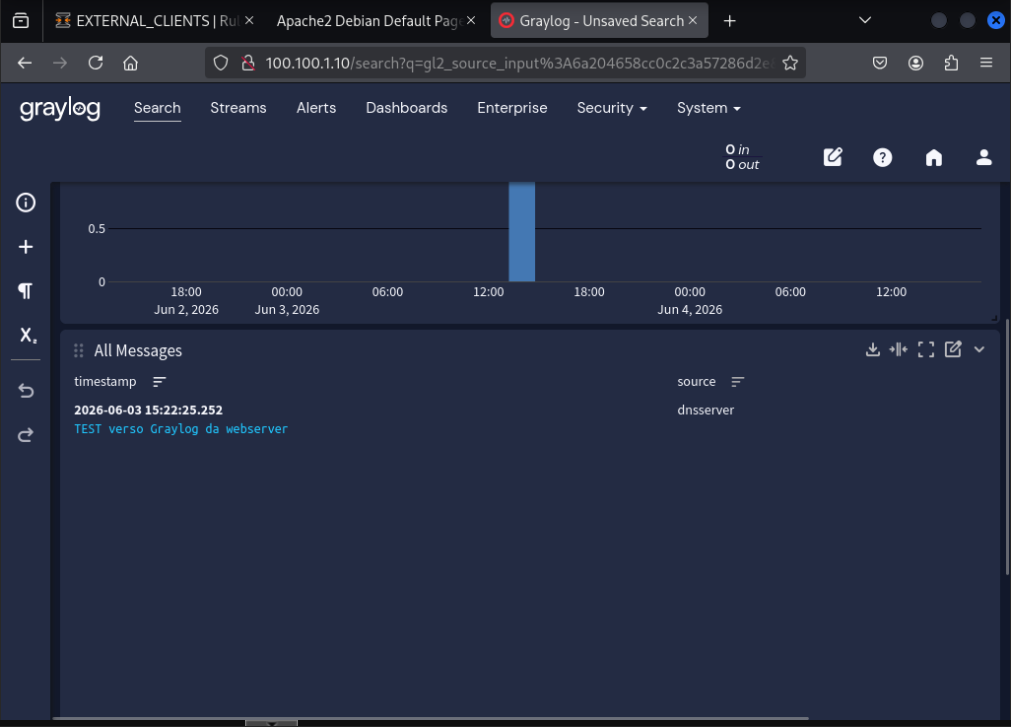
\includegraphics[width=\linewidth]{graylog_log_from_dnsserver.png}
\caption{Graylog receiving a remote log message (centralized logging).}
\label{fig:graylog}
\end{figure}

\section{Definition of the security policy}

The policy was written declaratively first. Table~\ref{tab:matrix} is the
inter-zone matrix (\textit{R} = allowed but restricted to the flows below,
\textit{D} = deny); Table~\ref{tab:flows} lists the flows that the firewalls
actually permit.

\begin{table}[H]
\centering
\setlength{\tabcolsep}{4pt}
\begin{tabular}{l|ccccc}
\toprule
src\,$\backslash$\,dst & INET & DMZ & EXT & SRV & CLI \\
\midrule
INET & --- & R   & D   & D   & D \\
DMZ  & R   & --- & R   & R   & D \\
EXT  & D   & R   & --- & R   & D \\
SRV  & R   & R$^{*}$ & R$^{*}$ & --- & R$^{*}$ \\
CLI  & D$^{\dagger}$ & R   & D   & R   & --- \\
\bottomrule
\end{tabular}
\caption{Zone matrix. R$^{*}$ from SRV = Greenbone scan / proxy / DNS only;
$^{\dagger}$ CLI$\to$INET only ICMP (no direct HTTP/HTTPS).}
\label{tab:matrix}
\end{table}

\begin{table}[H]
\centering
\setlength{\tabcolsep}{3pt}
\begin{tabular}{lll}
\toprule
\textbf{Source} & \textbf{Destination} & \textbf{Port} \\
\midrule
Internet        & reverse proxy   & 80/443 \\
External clients& reverse proxy   & 80/443 \\
Clients         & forward proxy   & 3128 \\
Clients         & reverse proxy   & 80/443 \\
Clients/DMZ/Ext & DNS server      & 53 \\
Clients/DMZ/Ext & log server      & 514, 6514 \\
Clients/DMZ/Ext & Graylog         & 5140, 12201 \\
Proxy           & Internet        & 80/443 \\
DNS server      & Internet        & 53 \\
Servers         & forward proxy   & 3128 \\
Greenbone       & all ACME zones  & any \\
admin (Kali)    & firewalls GUI / Greenbone / Graylog & mgmt \\
\bottomrule
\end{tabular}
\caption{Allowed \textit{application} flows. In addition, each interface permits
ICMP/ICMPv6 (diagnostics, NDP, PMTUD) and the firewalls forward their own logs
to Graylog (\texttt{100.100.254.1$\to$graylog:5140}); everything else is dropped
by default-deny.}
\label{tab:flows}
\end{table}

Three asymmetries are deliberate. Clients have \textit{no} direct Internet
HTTP/HTTPS (only via the proxy); ICMP toward the Internet is left open for
diagnostics, so \texttt{CLI$\to$INET} is a deny \textit{except} ping. Greenbone
\textit{initiates} the scans and never accepts connections, with the single
exception of the administrator reaching its web UI. Finally, the administrative
restriction is \textit{host-level}, not zone-level: the matrix shows
\texttt{CLI$\to$SRV = R} for the whole client network, but the rules pin the
management flows (firewall GUIs, Greenbone, Graylog UI) to the
\texttt{host\_admin} alias (Kali) only --- the zone matrix alone cannot express
this, the alias-based rules do.

\section{Policy implementation}

The matrix was implemented on both OPNsense firewalls. To keep the rules
readable we used \textbf{aliases} (\texttt{host\_webserver},
\texttt{host\_proxyserver}, \texttt{net\_dmz}, \texttt{port\_web}, \dots) instead
of raw addresses. On each interface the old permissive \texttt{any\,$\to$\,any}
rule was disabled and replaced by the explicit pass rules of
Table~\ref{tab:flows}, closed by a final \texttt{block log any\,$\to$\,any}.

\paragraph{Dual-stack.}
Because the network is dual-stack since Assignment~1, the service rules use
\texttt{inet46} (the OPNsense label for ``IPv4+IPv6'') and the aliases carry both the IPv4 address and the
IPv6 one; an explicit \textbf{ICMPv6} pass rule per interface allows the
essential types (NDP, PMTUD), as recommended by RFC~4890~\cite{rfc4890}. Without
it, IPv6 would break even though every service answers on IPv6.

\paragraph{Default-deny on every interface.}
Each interface (WAN, DMZ, External, Internal, Clients, Servers) ends with a
logging \texttt{block} rule. This both enforces the policy and produces the
evidence used in the tests.

\paragraph{Firewalls as log sources.}
Both firewalls forward their packet-filter logs to Graylog (Syslog UDP/5140), so
the pass/block decisions are centralized. Since the Main firewall must cross the
Internal one to reach Graylog, a dedicated pass rule
(\texttt{100.100.254.1\,$\to$\,graylog:5140}) was added on the Internal firewall.
Graylog receives \texttt{filterlog} events from both firewalls
(Figure~\ref{fig:fwlogs}).

\begin{figure}[H]
\centering
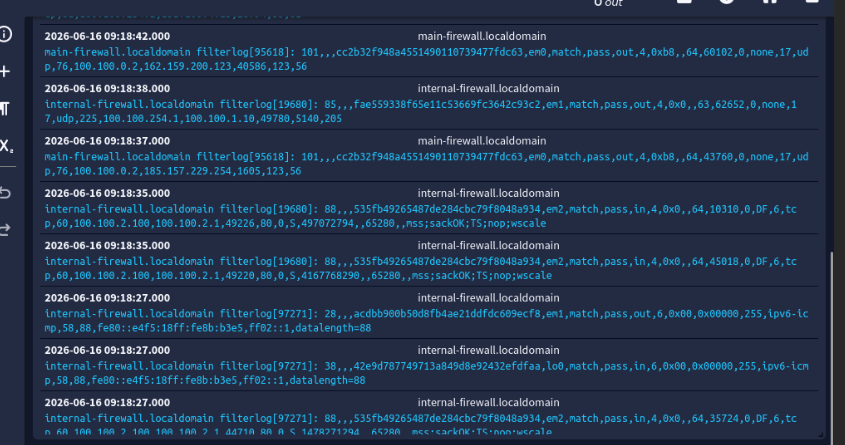
\includegraphics[width=\linewidth]{firewall_logs.png}
\caption{Filter logs of both firewalls collected in Graylog.}
\label{fig:fwlogs}
\end{figure}

\section{Test of the policy enforcement}

For every flow we checked that allowed traffic passes and forbidden traffic is
dropped and logged. The lab restricts Internet egress (only ping, plus an
HTTP/HTTPS domain whitelist), so reachability tests use a whitelisted domain
(\texttt{debian.org}).

\paragraph{Proxy and direct-egress block.}
From a client, browsing through Squid works while a direct connection to the
Internet times out, confirming the proxy-only policy:

\begin{lstlisting}
$ curl -x http://100.100.6.3:3128 -I https://debian.org
HTTP/1.1 200 Connection established  (Via: proxyserver)
$ curl -I https://debian.org --connect-timeout 5
# DENY / timeout (no direct egress)
\end{lstlisting}

\paragraph{Reverse proxy by name.}
After aligning DNS to the reverse proxy, internal clients reach the published
services \textit{by name}, transparently through nginx
(Figure~\ref{fig:dnscurl}); a \texttt{GET} on the vending machine returns its
real page (Figure~\ref{fig:coffee}).

\begin{figure}[H]
\centering
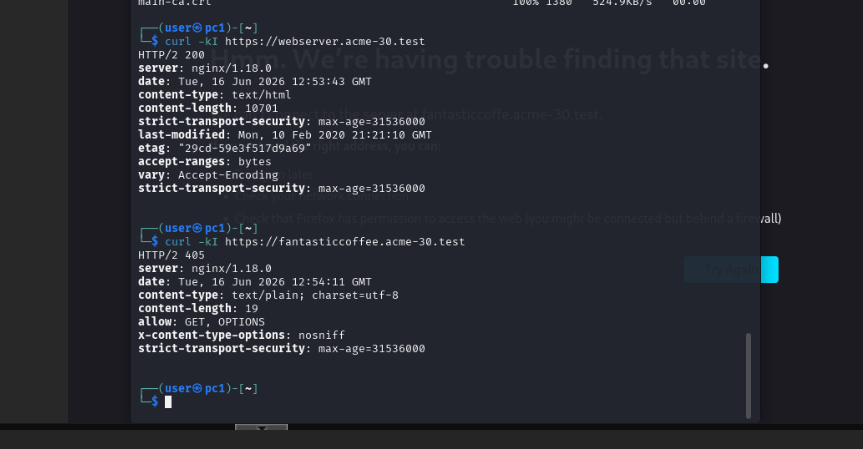
\includegraphics[width=\linewidth]{dns_reverseproxy_curl.png}
\caption{Clients reach the web service and the vending machine by name through
the reverse proxy (\texttt{server: nginx}).}
\label{fig:dnscurl}
\end{figure}

\begin{figure}[H]
\centering
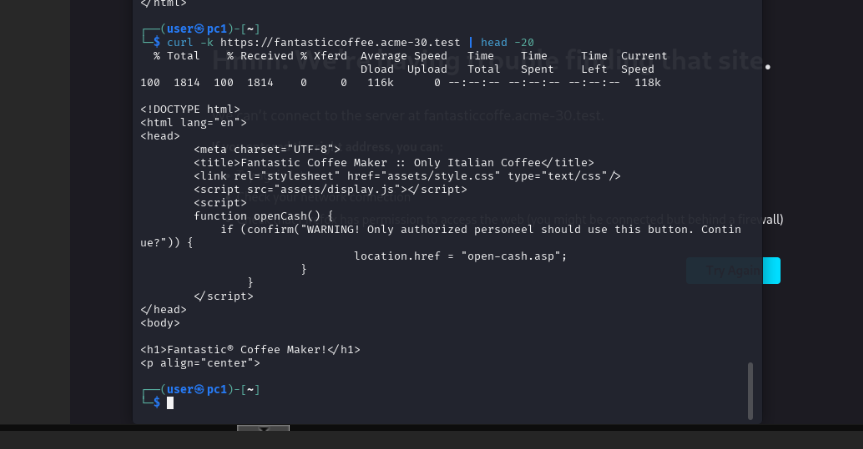
\includegraphics[width=\linewidth]{fantasticcoffee_get.png}
\caption{The vending machine page served end-to-end through the reverse proxy
over HTTPS.}
\label{fig:coffee}
\end{figure}

\paragraph{IPv6 enforcement.}
Name resolution and access to the reverse proxy work over IPv6 as well
(Figure~\ref{fig:v6}), while a direct connection to the backend is blocked,
confirming the dual-stack policy:

After the DNS alignment the AAAA record of the name points to the reverse
proxy (\texttt{...1e06:74da...}), so the client reaches it \textit{by name},
with no manual override:

\begin{lstlisting}
$ dig -6 webserver.acme-30.test AAAA +short
2001:470:b5b8:1e06:74da:b5ff:fed2:952a   # proxy
$ curl -6 -kI https://webserver.acme-30.test/
HTTP/2 200  (server: nginx/1.18.0)
\end{lstlisting}

\begin{figure}[H]
\centering
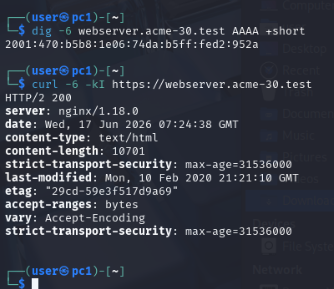
\includegraphics[width=\linewidth]{fromkali_v6test.png}
\caption{IPv6 end-to-end test from a client: AAAA resolution and access to the
reverse proxy over IPv6.}
\label{fig:v6}
\end{figure}

\paragraph{Internet $\to$ reverse proxy.}
From a host on the simulated Internet (no VPN), the published services are
reachable \textit{only} through the reverse proxy, while the real backends are
not. The proxy presents the internal-CA certificate (TLS terminated there):

\newpage

\begin{lstlisting}
$ curl -k --resolve webserver.acme-30.test:443:\
    100.100.6.3 -I https://webserver.acme-30.test/
HTTP/2 200   (server: nginx/1.18.0)
$ ... s_client ... | openssl x509 -subject -issuer
subject= CN=webserver.acme-30.test
issuer = CN=internal-ca
$ curl -k --connect-timeout 5 -I https://100.100.6.2/
curl: (28) Connection timed out      # backend: DENY
$ nc -znv -w3 100.100.1.4 9392
... timed out                         # Greenbone: DENY
\end{lstlisting}

The firewall log confirms it: from the same Internet host, the request to the
proxy (\texttt{.6.3:443}) passes while the ones to the backend
(\texttt{.6.2:443}) are dropped (Figure~\ref{fig:wanrev}).

\begin{figure}[H]
\centering
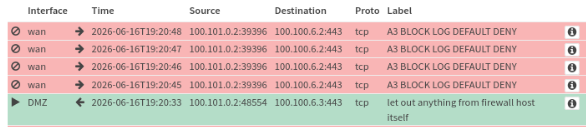
\includegraphics[width=\linewidth]{wan_to_reverseproxy.png}
\caption{Internet host: traffic to the reverse proxy (\texttt{.6.3}) is allowed,
direct traffic to the backend (\texttt{.6.2}) is dropped.}
\label{fig:wanrev}
\end{figure}

\paragraph{Default-deny logging.}
Forbidden traffic (e.g.\ an Internet host probing the firewall or an internal
backend) is dropped and logged by the \texttt{BLOCK LOG DEFAULT DENY} rule, as
shown in the firewall live view (Figure~\ref{fig:block}).

\begin{figure}[H]
\centering
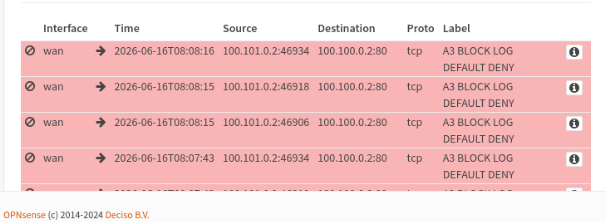
\includegraphics[width=\linewidth]{blocking_traffic.png}
\caption{Traffic not matching any allow rule is dropped and logged.}
\label{fig:block}
\end{figure}

\paragraph{Administration.}
The firewall GUIs, the Greenbone UI (9392) and the Graylog UI are reachable from
the admin host (Kali) and denied to ordinary clients. Greenbone can scan the
ACME zones, and the \textit{only} connection accepted toward it is the
administrator reaching its UI: no other host may initiate any connection to the
scanner.

\section{Final remarks}

The ACME network now enforces a coherent \textit{least-privilege, default-deny}
policy on both firewalls: every allowed flow maps to one readable, alias-based
rule, every other packet is dropped and logged, and the dropped events are
centralized in Graylog together with the host and service logs. Public web
services are exposed only through a single reverse proxy that upgrades them to
HTTPS, internal hosts reach the Internet only through the forward proxy, and the
whole policy was replicated on IPv6.

A few hardening steps were already applied beyond the minimum (HTTPS-only web
service, syslog over TLS, ICMPv6 filtering, firewall log forwarding).

\begin{thebibliography}{9}

\bibitem{nist80041}
K.~Scarfone, P.~Hoffman,
\textit{Guidelines on Firewalls and Firewall Policy},
NIST SP~800-41 Rev.\,1, 2009.

\bibitem{rfc4890}
E.~Davies, J.~Mohacsi,
\textit{Recommendations for Filtering ICMPv6 Messages in Firewalls},
RFC~4890, 2007.

\bibitem{rfc5425}
F.~Miao, Y.~Ma, J.~Salowey,
\textit{Transport Layer Security (TLS) Transport Mapping for Syslog},
RFC~5425, 2009.

\end{thebibliography}

\begin{figure*}[!t]
\centering
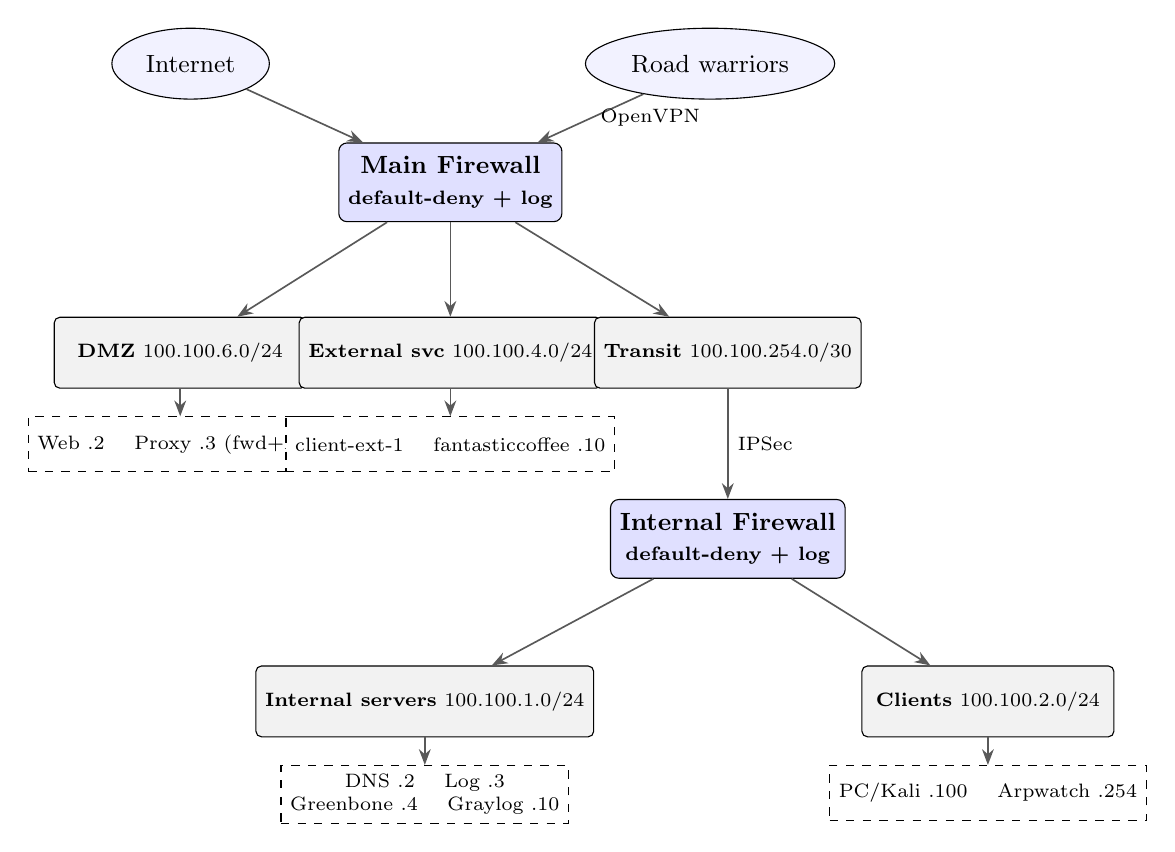
\begin{tikzpicture}[
  font=\sffamily,
  node distance=0.9cm and 1.1cm,
  fw/.style={draw, rounded corners=3pt, fill=blue!12, minimum width=2.8cm,
             minimum height=1cm, align=center, font=\small\bfseries},
  net/.style={draw, fill=gray!10, rounded corners=2pt, minimum width=3.2cm,
              minimum height=0.9cm, align=center, font=\scriptsize},
  host/.style={draw, dashed, fill=white, minimum width=3.2cm,
               minimum height=0.7cm, align=center, font=\scriptsize},
  cloud/.style={draw, ellipse, fill=blue!5, minimum width=2cm,
                minimum height=0.9cm, font=\small},
  link/.style={-Stealth, semithick, draw=black!65},
]

\node[cloud] (inet) {Internet};
\node[cloud, right=4cm of inet] (rw) {Road warriors};

\node[fw, below=1cm of $(inet)!0.5!(rw)$] (mfw)
    {Main Firewall \\ \scriptsize default-deny + log};

\node[net, below left=1.2cm and 0.4cm of mfw] (dmz)
    {\textbf{DMZ} 100.100.6.0/24};
\node[net, below=1.2cm of mfw] (ext)
    {\textbf{External svc} 100.100.4.0/24};
\node[net, below right=1.2cm and 0.4cm of mfw] (link)
    {\textbf{Transit} 100.100.254.0/30};

\node[host, below=0.35cm of dmz] (dmzh)
    {Web .2 \quad Proxy .3 (fwd+rev)};
\node[host, below=0.35cm of ext] (exth)
    {client-ext-1 \quad fantasticcoffee .10};

\node[fw, below=1.4cm of link] (ifw) {Internal Firewall \\ \scriptsize default-deny + log};

\node[net, below left=1.1cm and 0.2cm of ifw] (srv)
    {\textbf{Internal servers} 100.100.1.0/24};
\node[net, below right=1.1cm and 0.2cm of ifw] (cli)
    {\textbf{Clients} 100.100.2.0/24};

\node[host, below=0.35cm of srv] (srvh)
    {DNS .2 \quad Log .3 \\ Greenbone .4 \quad Graylog .10};
\node[host, below=0.35cm of cli] (clih)
    {PC/Kali .100 \quad Arpwatch .254};

\draw[link] (inet) -- (mfw);
\draw[link] (rw) -- node[midway, right, font=\scriptsize] {OpenVPN} (mfw);
\draw[link] (mfw) -- (dmz);
\draw[link] (mfw) -- (ext);
\draw[link] (mfw) -- (link);
\draw[link] (dmz) -- (dmzh);
\draw[link] (ext) -- (exth);
\draw[link] (link) -- node[midway, right, font=\scriptsize] {IPSec} (ifw);
\draw[link] (ifw) -- (srv);
\draw[link] (ifw) -- (cli);
\draw[link] (srv) -- (srvh);
\draw[link] (cli) -- (clih);

\end{tikzpicture}
\caption{ACME-30 topology. The Main firewall protects the WAN/DMZ/External
zones and terminates the road-warrior VPN; the Internal firewall isolates the
servers and clients networks. Public web services are exposed only through the
reverse proxy in the DMZ.}
\label{fig:topology}
\end{figure*}

\end{document}
